%!TEX root = ../../../../report.tex
\subsection{Computer-Aided Design (CAD)} % (fold)
\label{sub:computer_aided_design}
After producing a final sketch for each component of the frame, the software SolidWorks was utilized to create their actual structure based on the required configuration, the desired placement of the sensors/actuators and wiring and the mechanical constraints calculated.
In the absence of precise data about the physical requirements of a component, its volume has been increased to reinforce the resistance of the piece.
When no mechanical or morphological constraints were to be applied, the criteria in CAD design has been mostly aesthetic, since the stile of the robot is worth considering, even if it does not influence its performance.

The CAD design has been carried out oriented to 3D-print manufacturing of the pieces, which adds new constraints in terms of resolution, size and materials available.
Some corrections had to be applied to the tolerances of the internal holes as explained in the section \ref{sub:arc_compensation} in order to avoid backslash.
However, the advantages of employing 3D printers for the construction of the prototype compensate for these limitations.

The implementation of the CAD design can be considered partially parametric due to the fact that a file with some parameters has been used in several parts.
This works so that in the reconstruction of the part, SolidWords reads the file and changes everything according to its content.
This has eased the iterative process of optimization of the manufactured components.
The values utilized are shown in the appendix \ref{app:cad_parameters}.
The results can be seen in the figures from \ref{fig:left_foot} to \ref{fig:knee_upper}.

\begin{figure}[ht!]
    \centering
    \begin{subfigure}[b]{0.49\textwidth}
        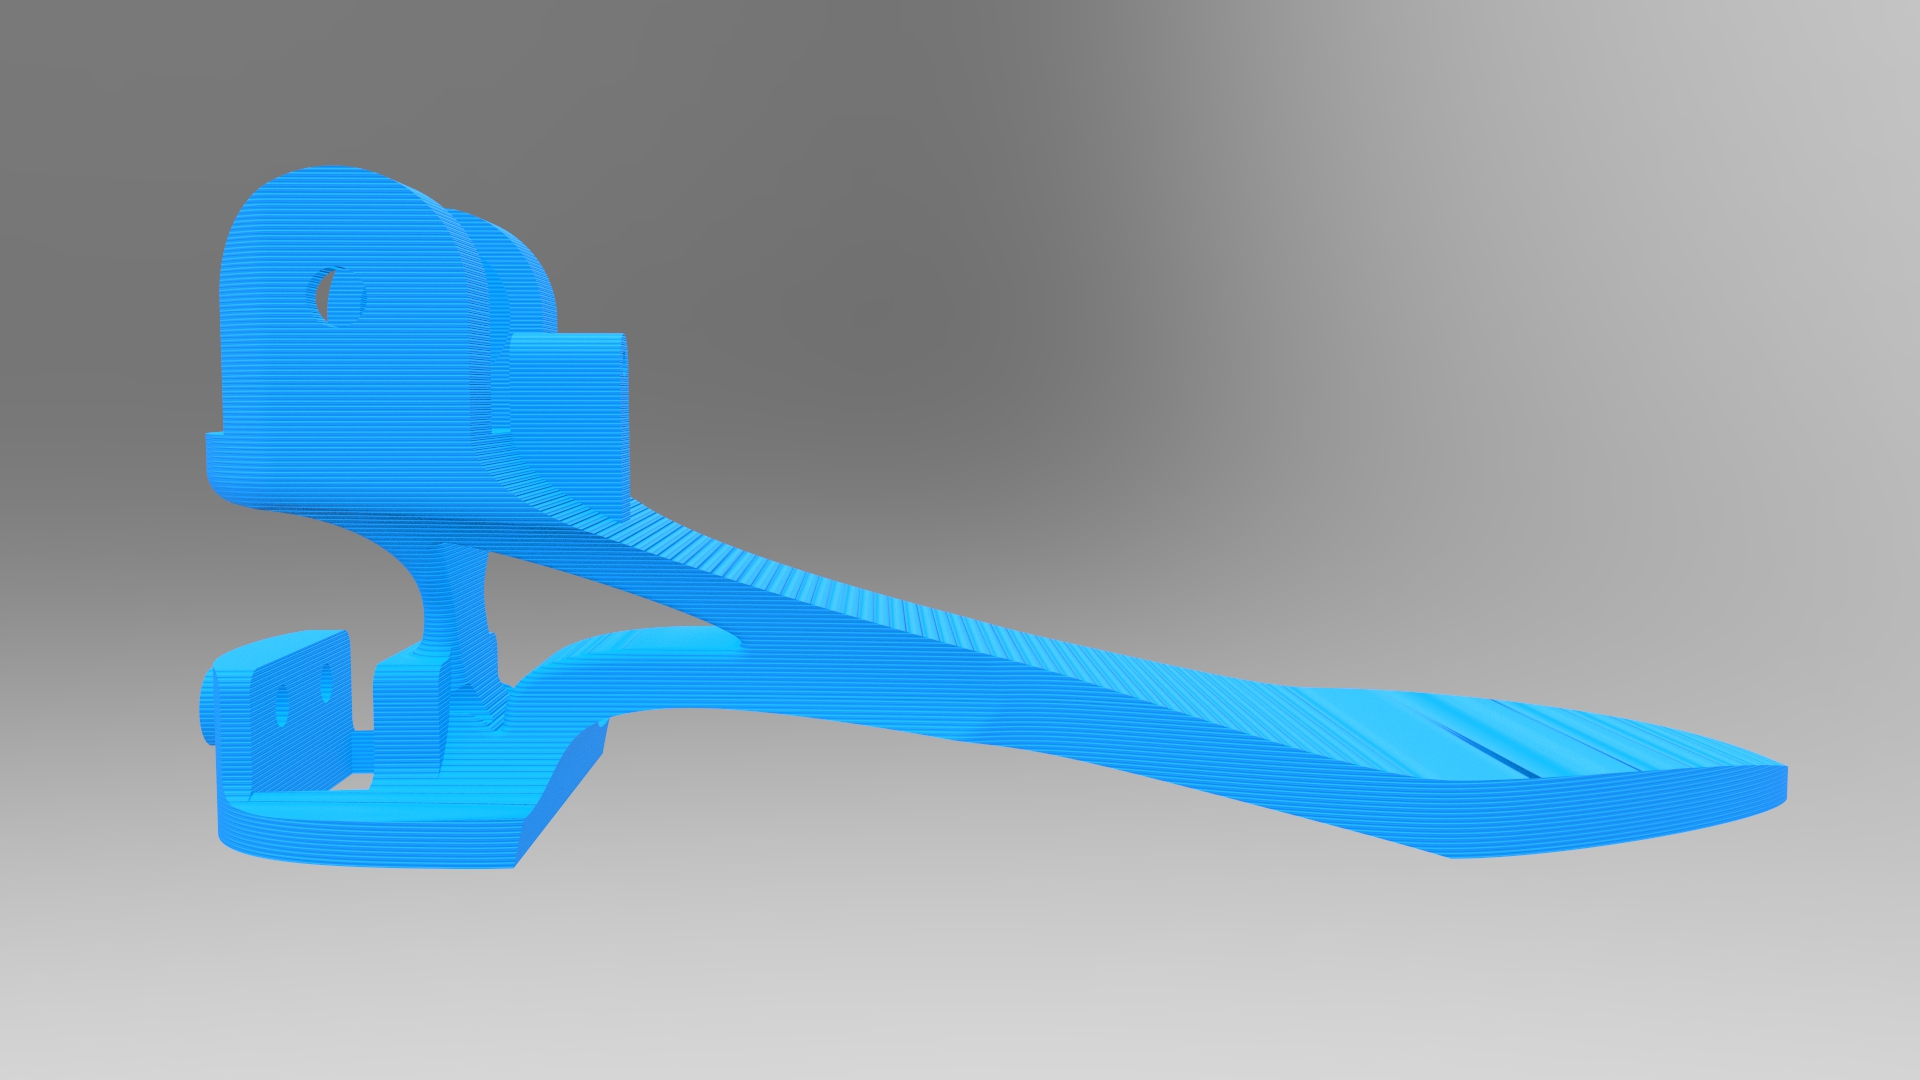
\includegraphics[width=\textwidth]{figures/legs_foot.jpg}
        \caption{Left foot}
        \label{fig:left_foot}
    \end{subfigure}
    \begin{subfigure}[b]{0.49\textwidth}
        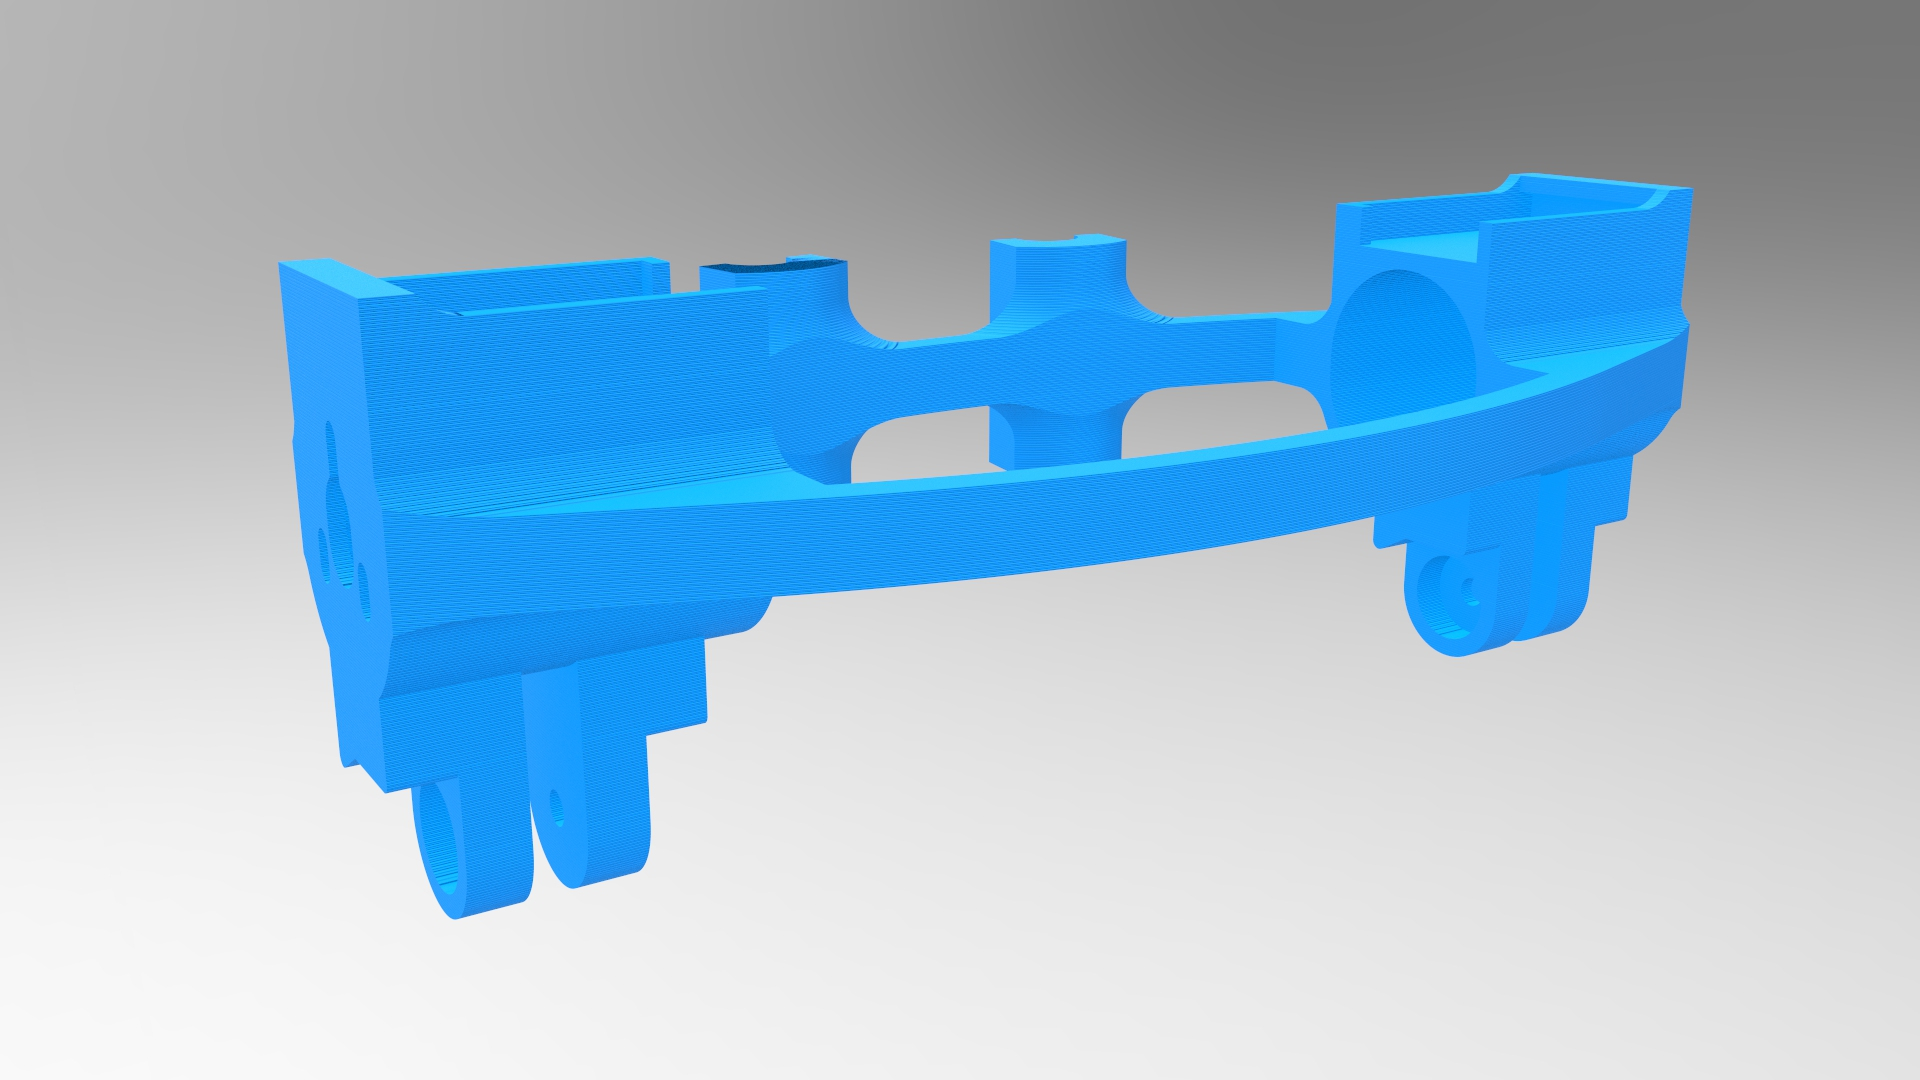
\includegraphics[width=\textwidth]{figures/legs_hip.jpg}
        \caption{Hip}
        \label{fig:hip}
    \end{subfigure}
\end{figure}    

\begin{figure}[ht!]
    \ContinuedFloat % continue from previous page
    \begin{subfigure}[b]{0.49\textwidth}
        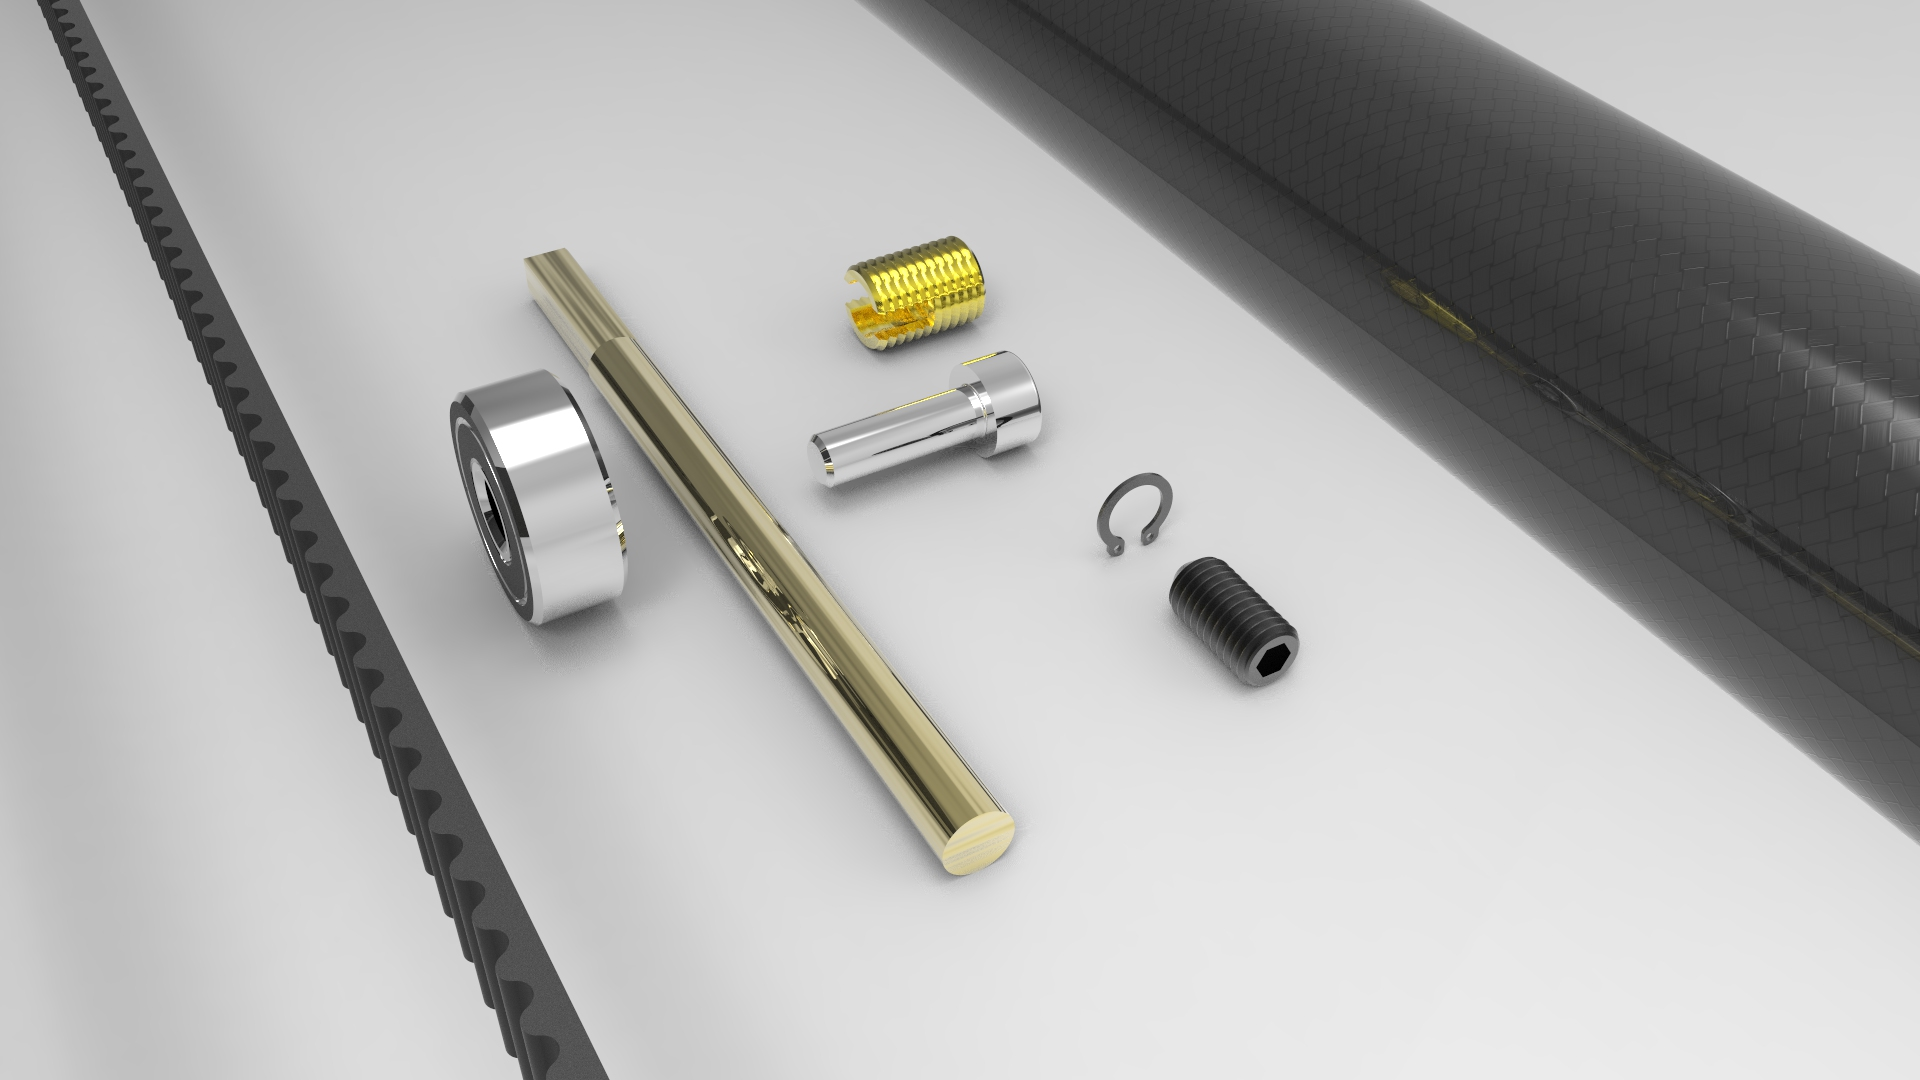
\includegraphics[width=\textwidth]{figures/legs_parts.jpg}
        \caption{Additional designed parts}
        \label{fig:mouse}
    \end{subfigure}
    \begin{subfigure}[b]{0.49\textwidth}
        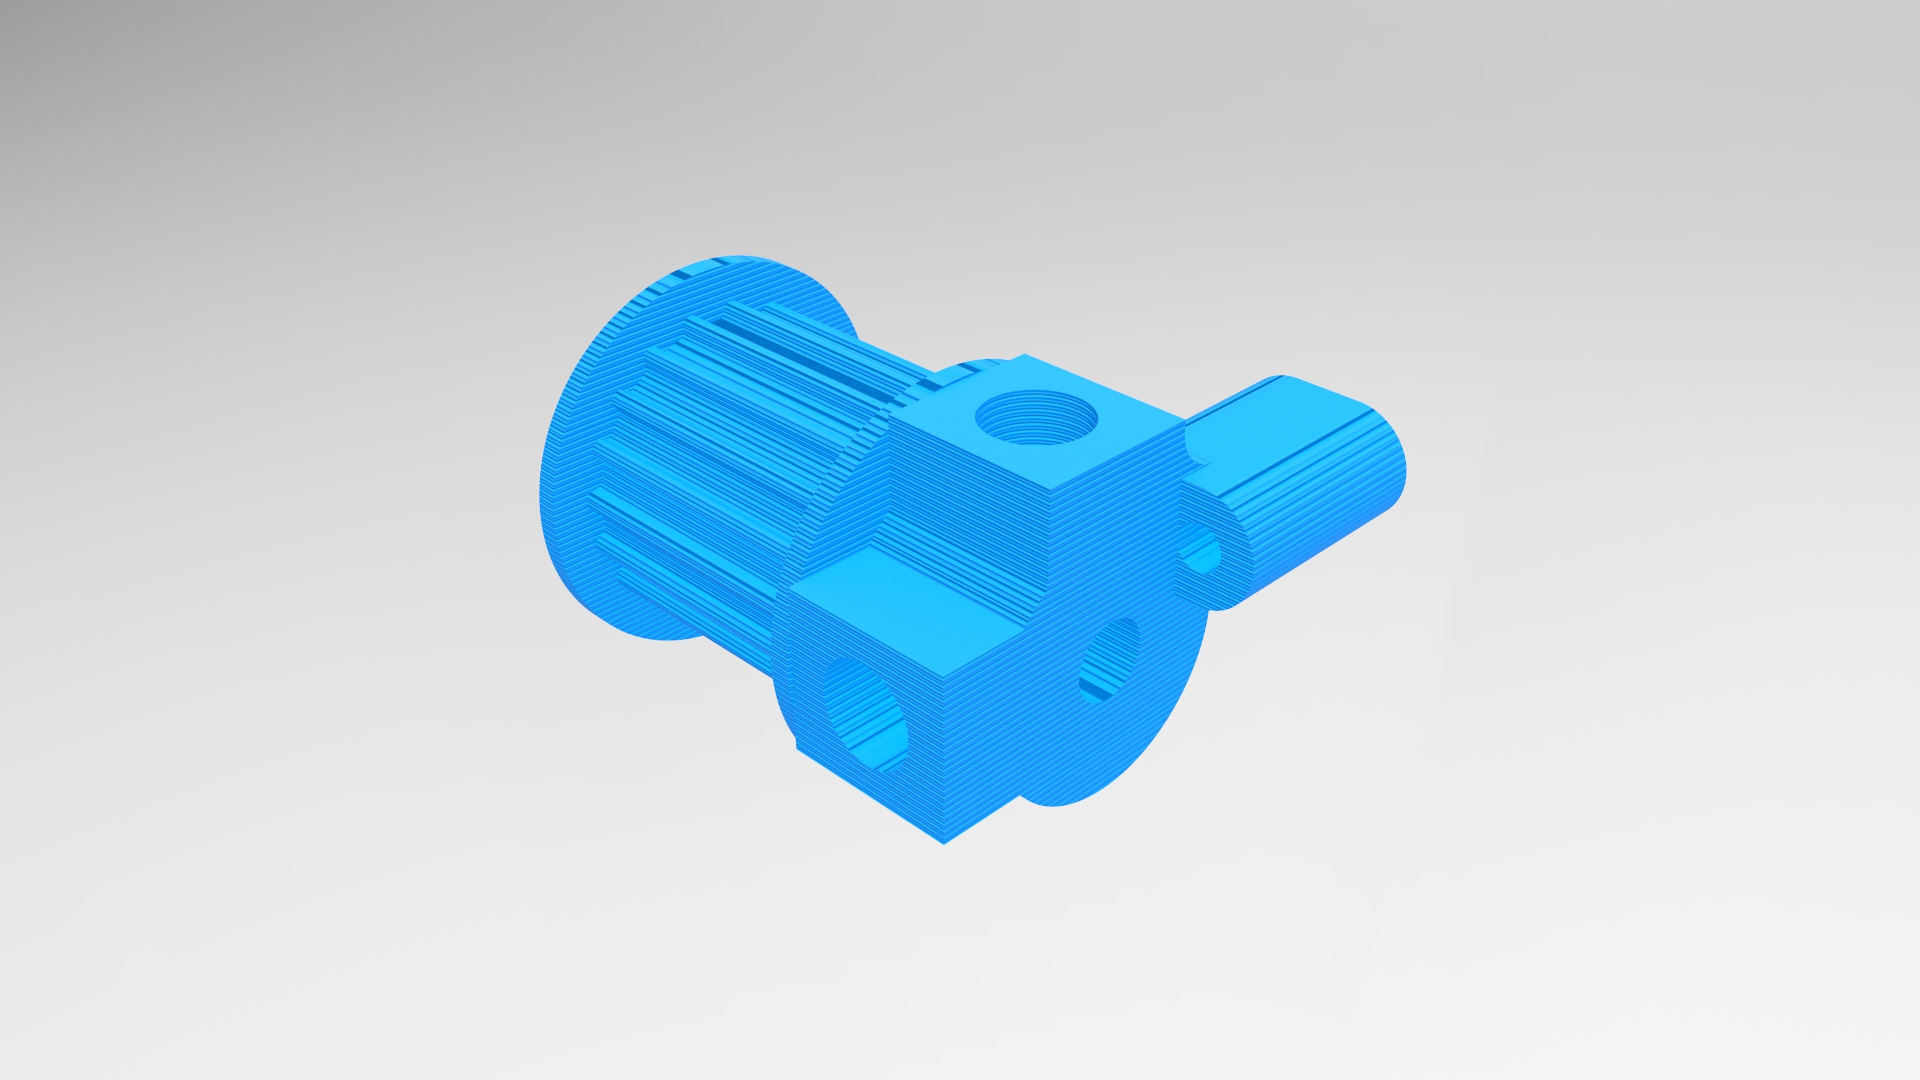
\includegraphics[width=\textwidth]{figures/legs_pulley.jpg}
        \caption{Left ankle serial spring pulley}
        \label{fig:serial_spring_pulley}
    \end{subfigure}
\end{figure}    

\begin{figure}[ht!]
    \ContinuedFloat % continue from previous page
    \begin{subfigure}[b]{0.49\textwidth}
        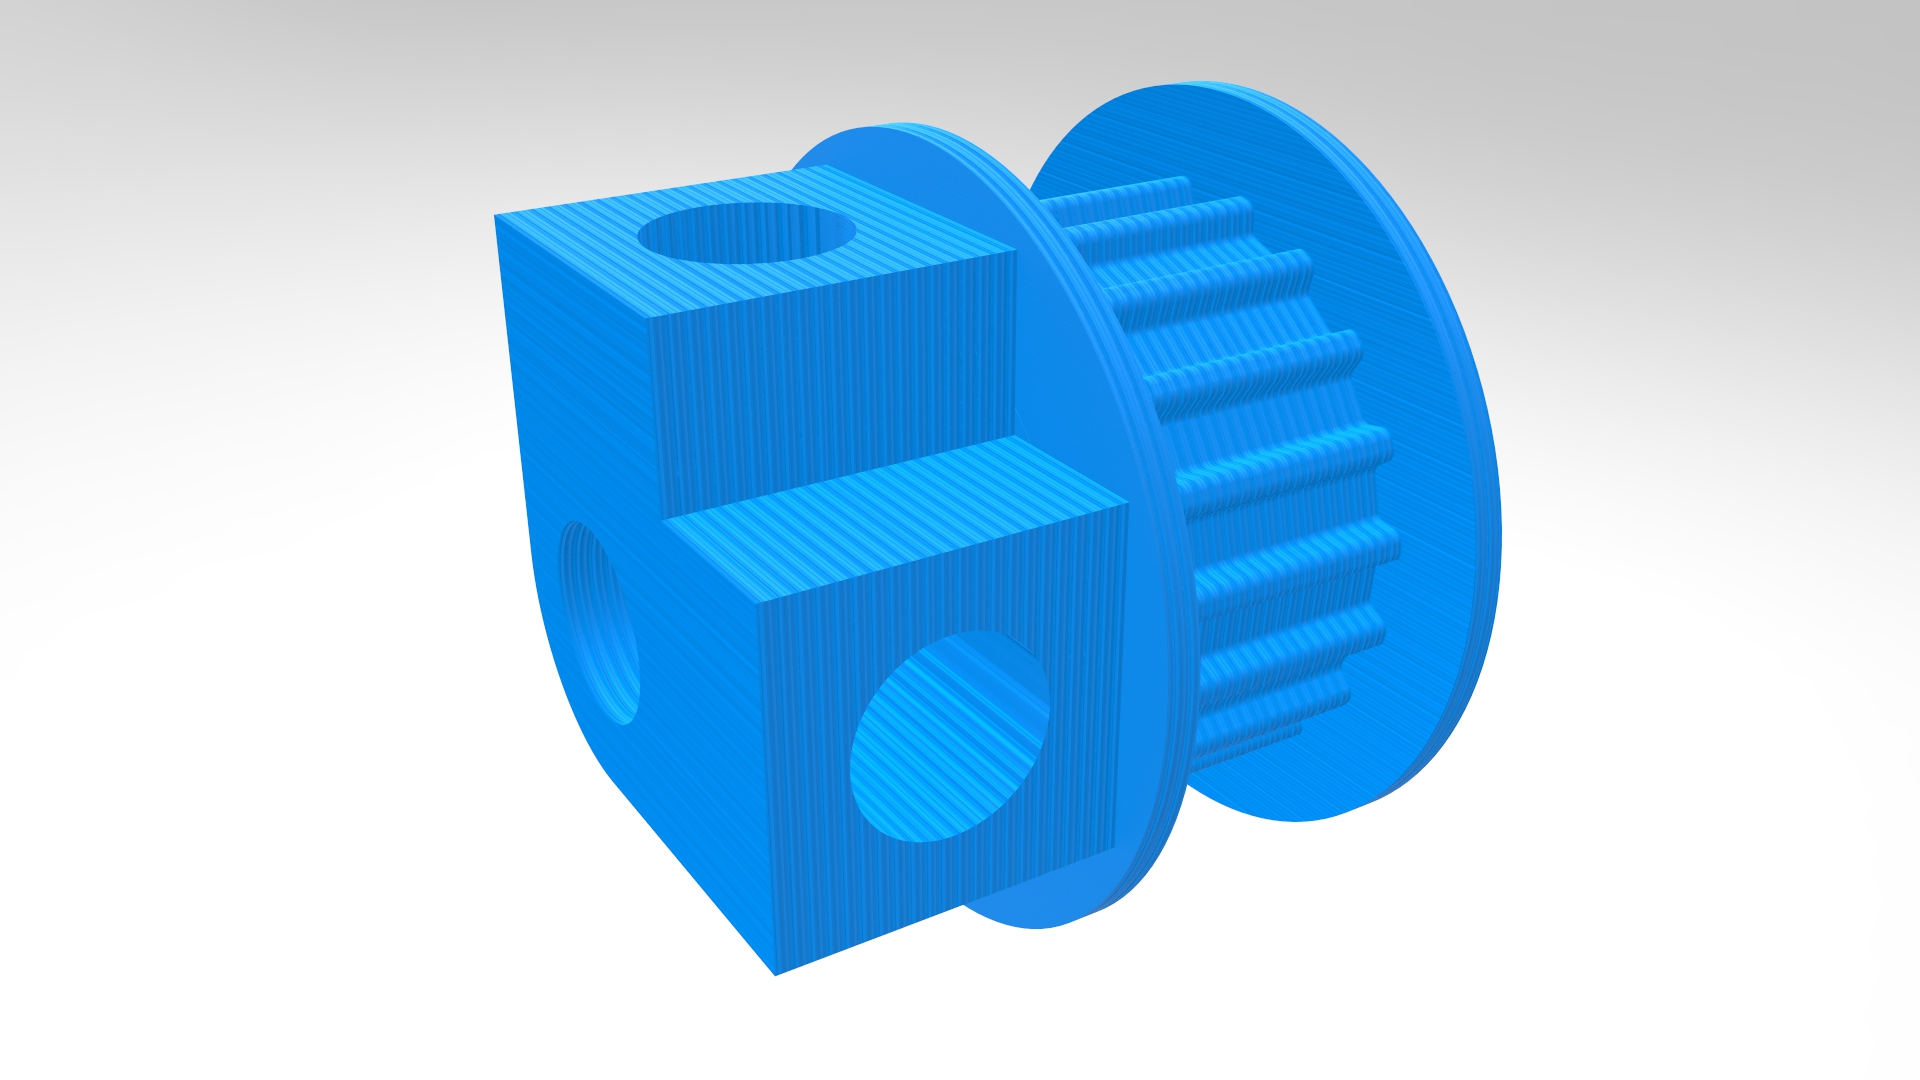
\includegraphics[width=\textwidth]{figures/legs_pulley_motor.jpg}
        \caption{Motor pulley}
        \label{fig:motor_pulley}
    \end{subfigure}
    \begin{subfigure}[b]{0.49\textwidth}
        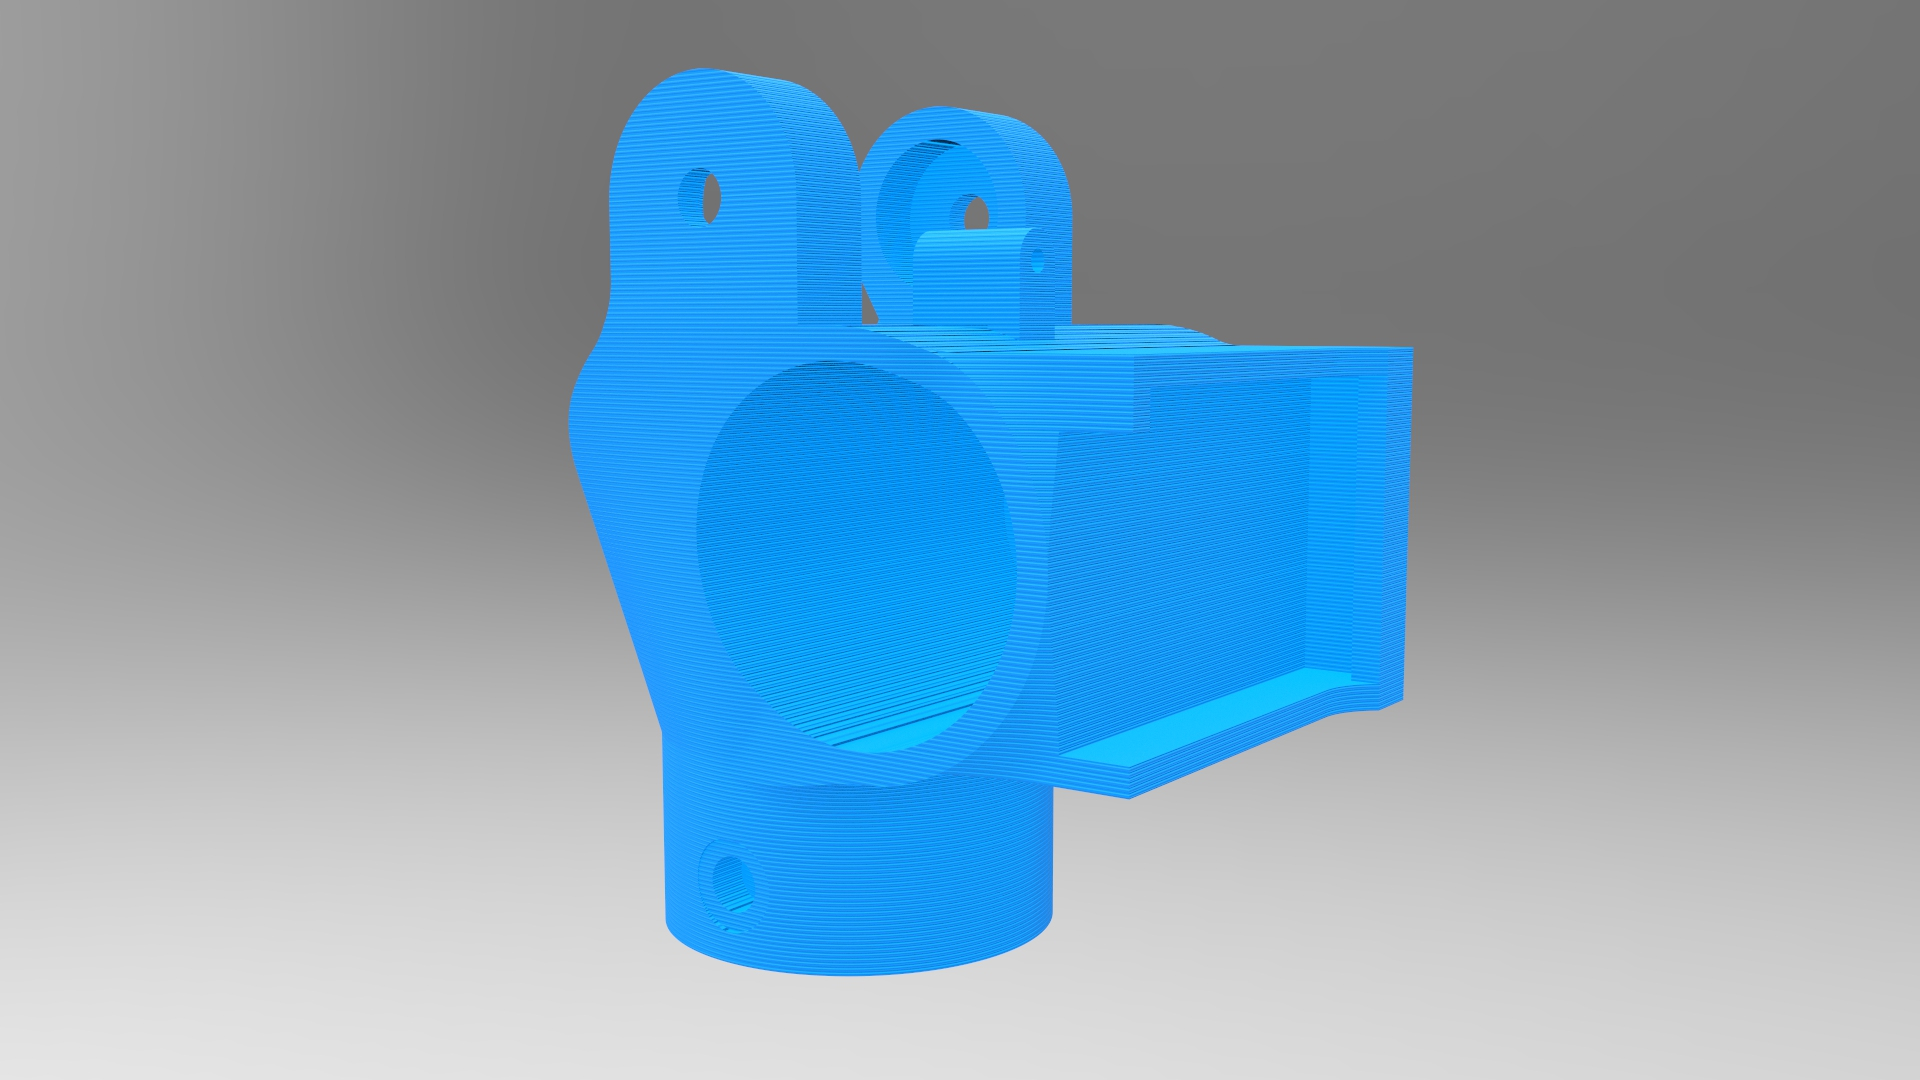
\includegraphics[width=\textwidth]{figures/legs_knee_lower.jpg}
        \caption{Left lower knee}
        \label{fig:lower_knee}
    \end{subfigure}
\end{figure}

\begin{figure}[ht!]
    \ContinuedFloat % continue from previous page
    \begin{subfigure}[b]{0.49\textwidth}
        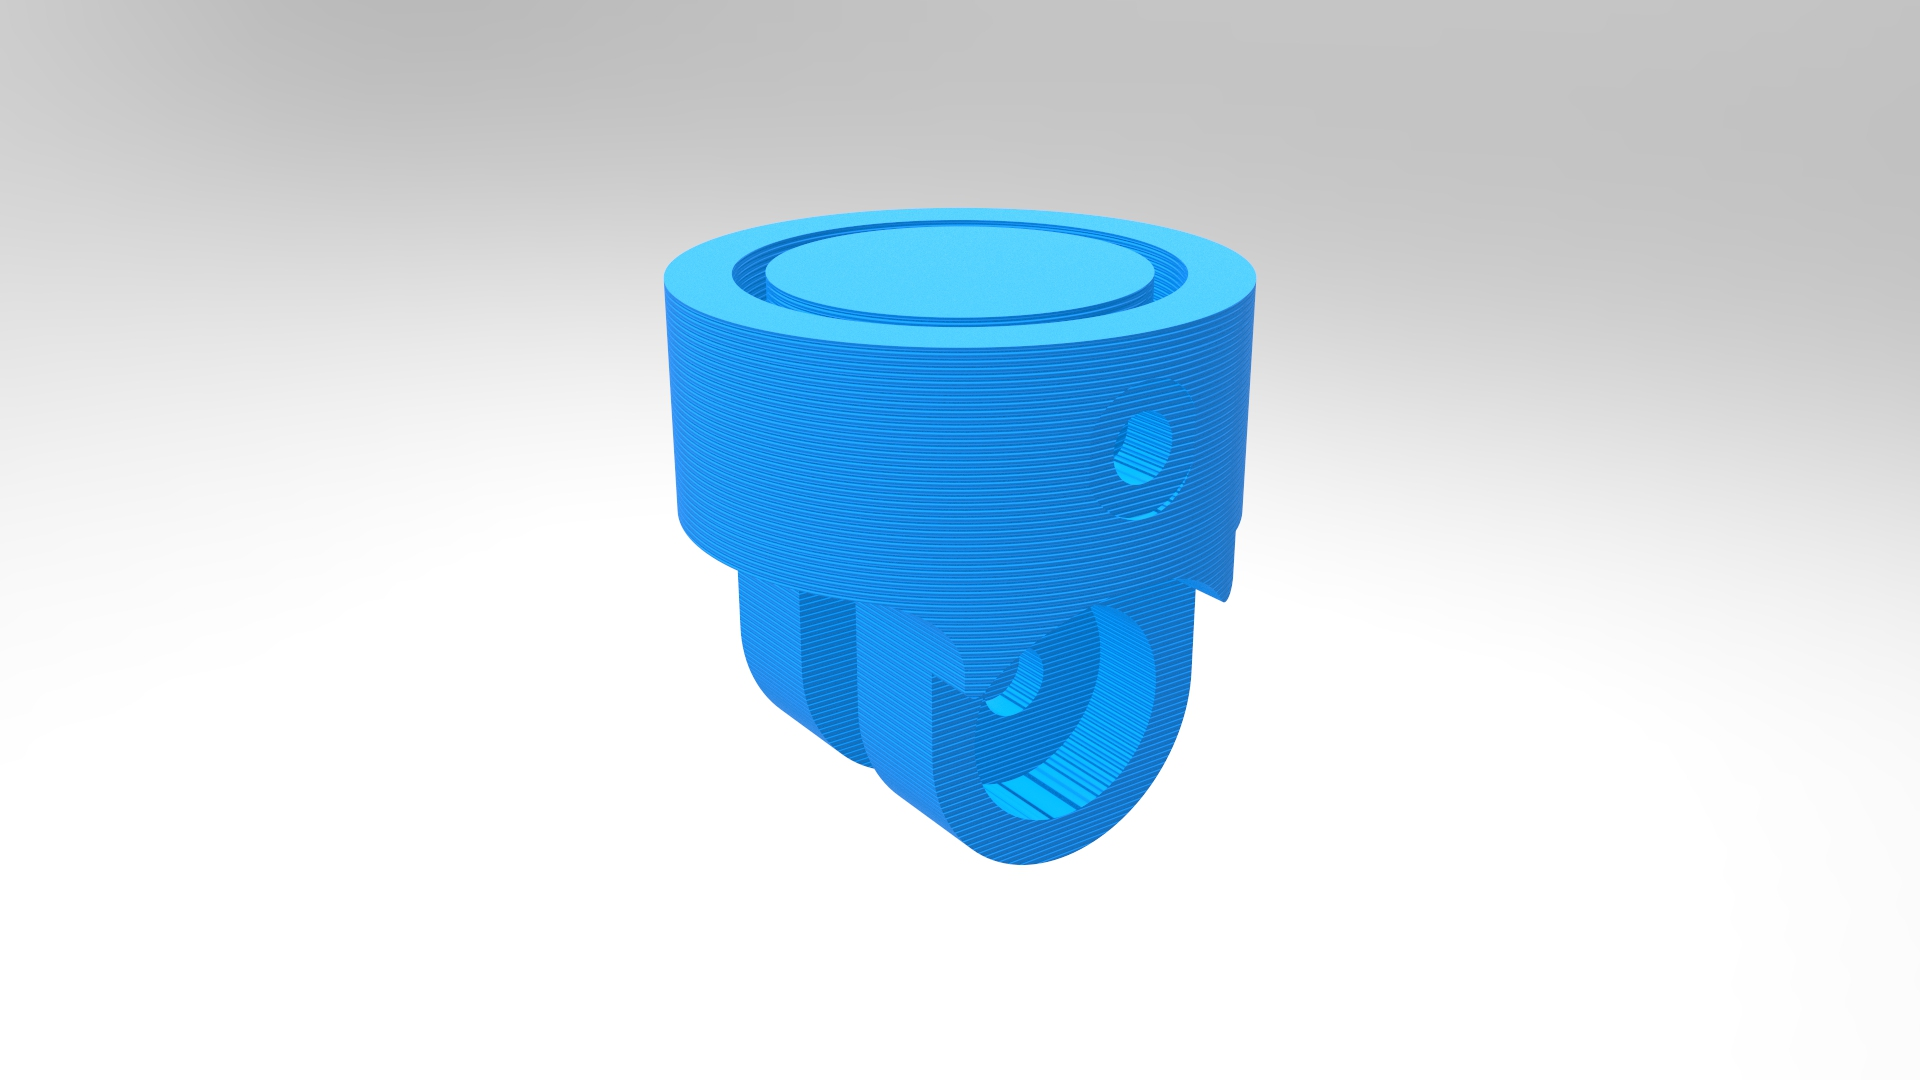
\includegraphics[width=\textwidth]{figures/legs_ankle_upper.jpg}
        \caption{Left upper ankle}
        \label{fig:ankle_upper}
    \end{subfigure}
    \begin{subfigure}[b]{0.49\textwidth}
        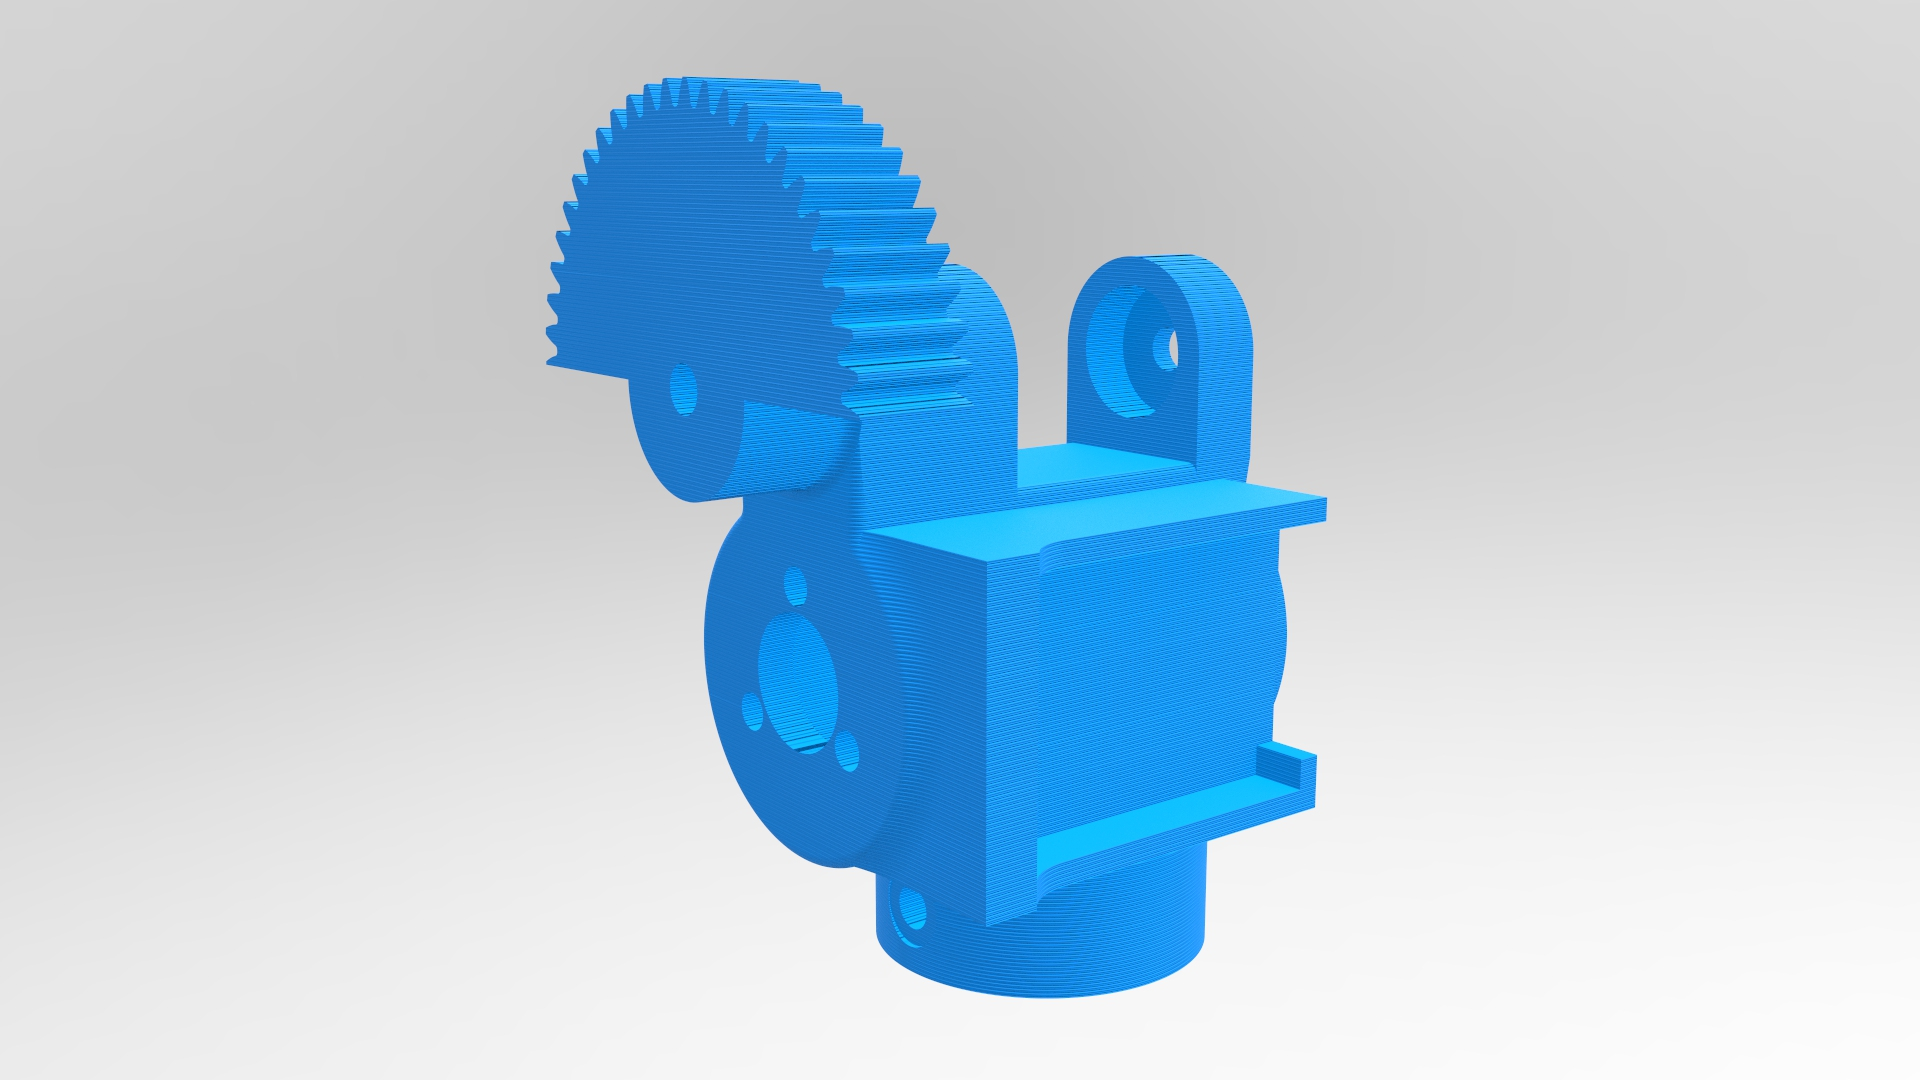
\includegraphics[width=\textwidth]{figures/legs_hip_lower.jpg}
        \caption{Left lower hip}
        \label{fig:hip_lower}
    \end{subfigure}
\end{figure}

\begin{figure}[ht!]
    \ContinuedFloat % continue from previous page
    \begin{subfigure}[b]{0.49\textwidth}
        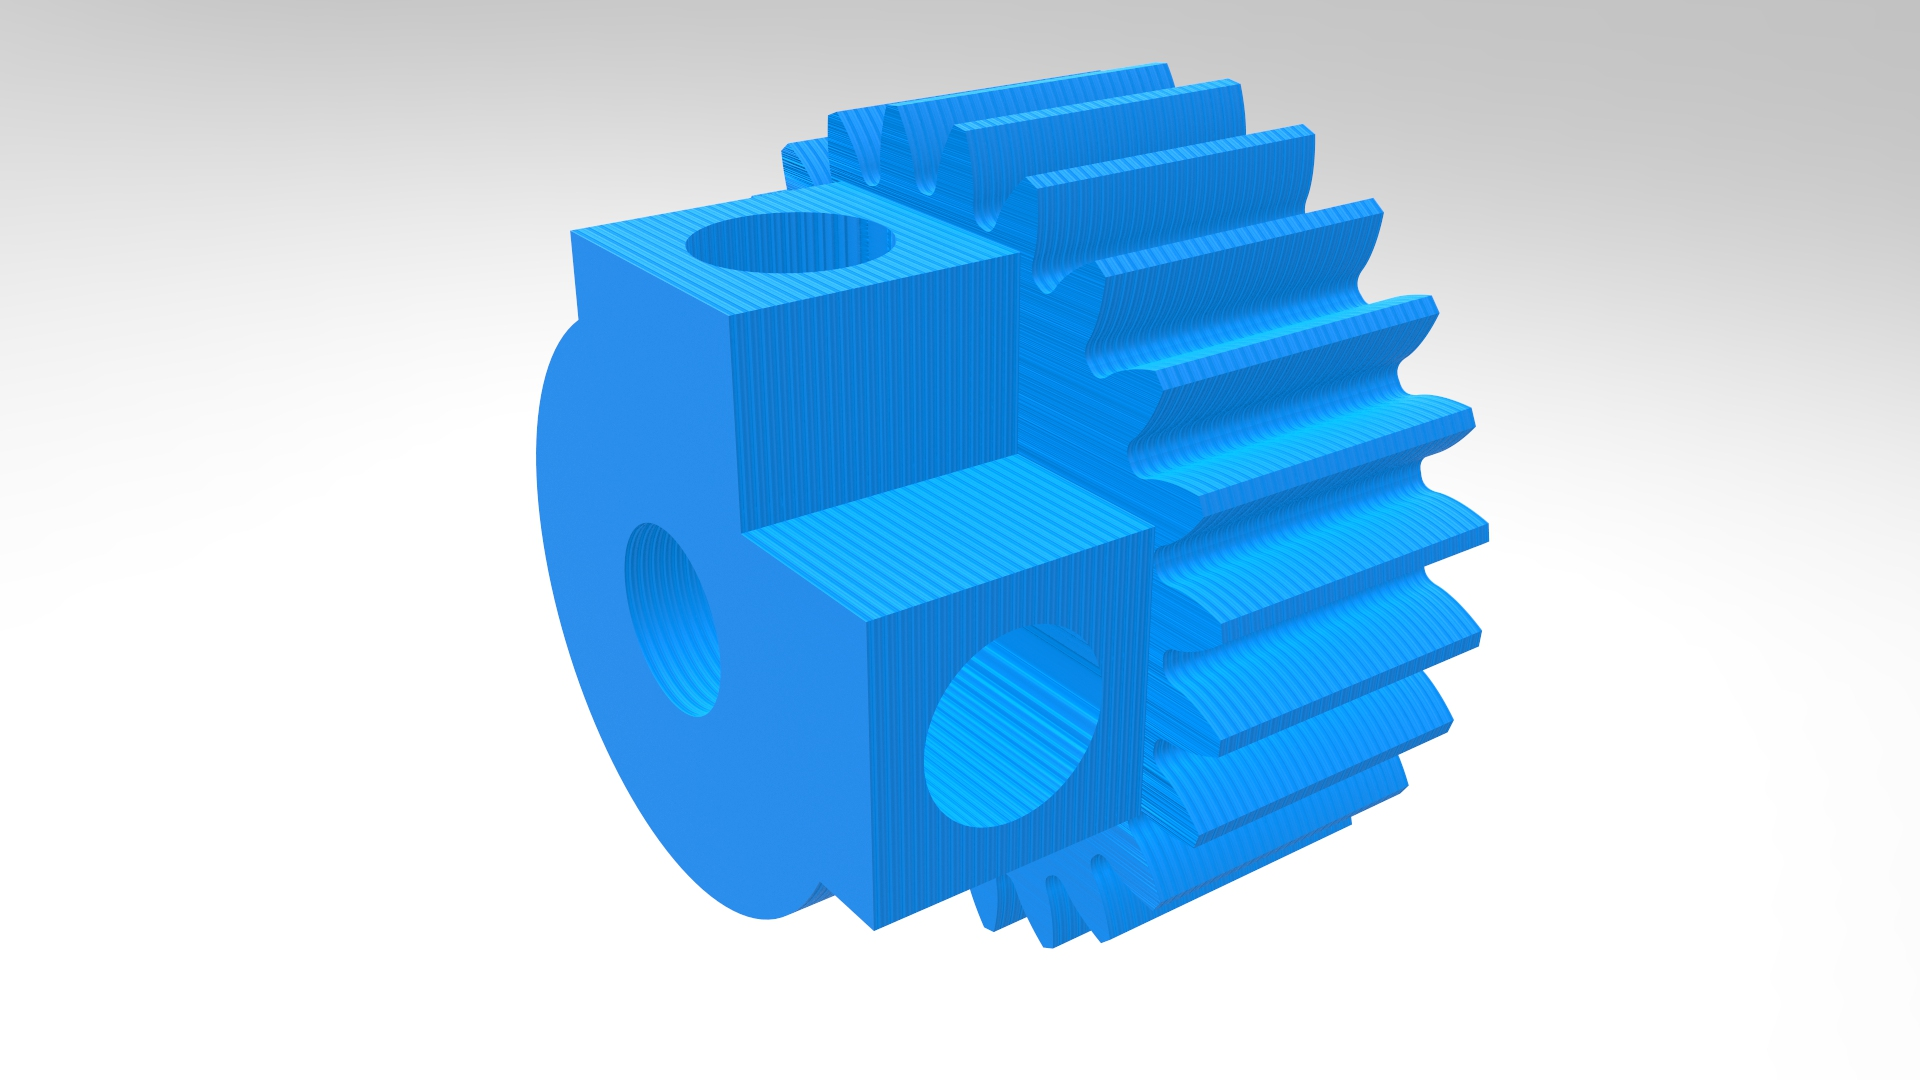
\includegraphics[width=\textwidth]{figures/legs_hip_pinion.jpg}
        \caption{Hip's pinion}
        \label{fig:hip_pinion}
    \end{subfigure}
    \begin{subfigure}[b]{0.49\textwidth}
        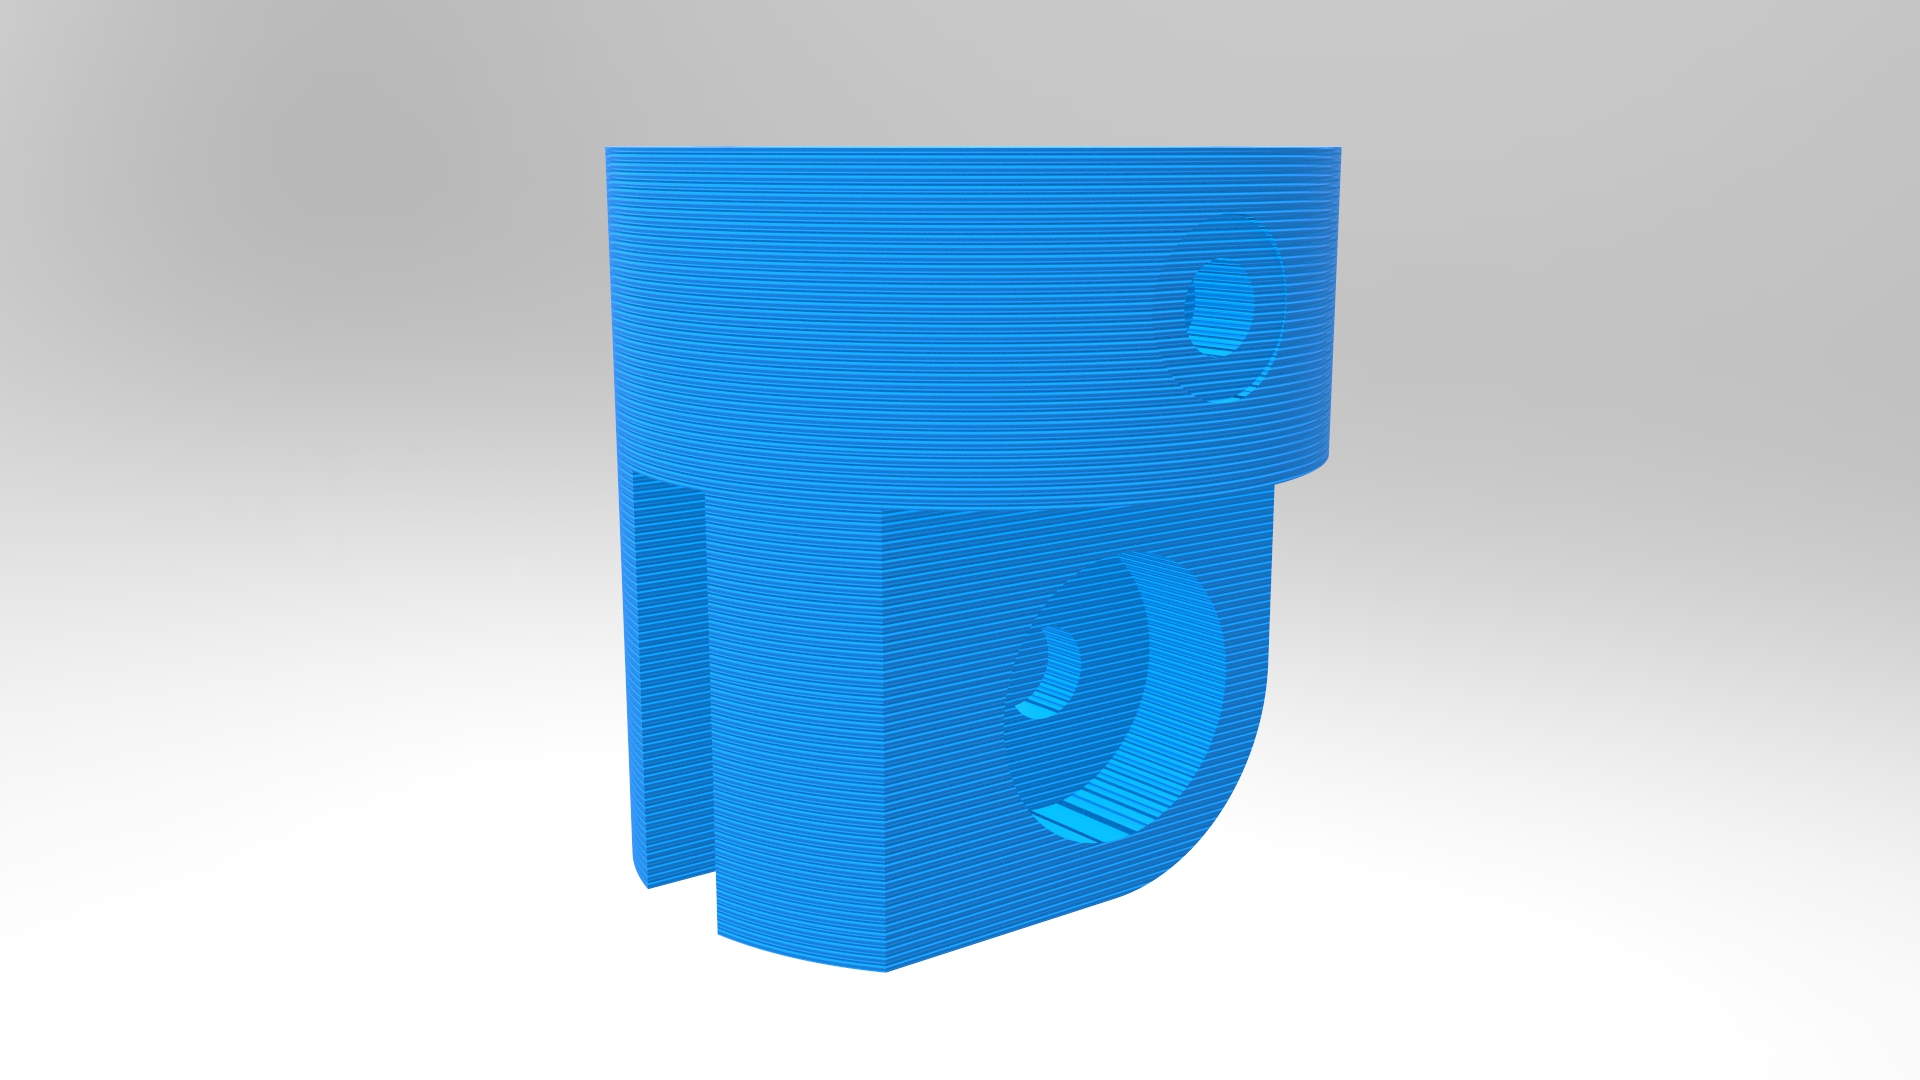
\includegraphics[width=\textwidth]{figures/legs_knee_upper.jpg}
        \caption{Left upper knee}
        \label{fig:knee_upper}
    \end{subfigure}
    \caption{Main CAD designed components}
\end{figure}

The CAD program has the feature of, given the physical properties of the materials used, calculate the geometrical values of a component such as moments of inertia or CoM position.
This has been used in the construction and use of the mathematical model in \ref{cha:mathematical_model} and to size the motors, or in the simulation \ref{cha:simulation} to create the model as close to reality as possible.
The tables from \ref{tab:foot_physical_properties} to \ref{tab:total_mass} contain the moments of inertia and total mass calculated by the CAD program.
The moments of inertia are taken from the appropriate rotation axis of the link.

\begin{table}[htbp]
\caption{Physical properties of the foot obtained from CAD program}
\begin{center}
\begin{tabular}{c|l|l}
\multicolumn{ 3}{c}{\Large \textbf{Foot}} \\
\multicolumn{ 3}{c}{\textbf{Mass $[Kg]$}} \\ \hline
\multicolumn{ 3}{c}{0.021} \\ \hline
\multicolumn{ 3}{c}{\textbf{Moments of inertia [$Kg \cdot m^2$] (Taken at output coordinate system)}} \\ \hline
Ixx = 2.2e-005 & \multicolumn{1}{c|}{Ixy = -9.16e-006} & \multicolumn{1}{c}{Ixz = 0} \\ \hline
Iyx = -9.16e-006 & \multicolumn{1}{c|}{Iyy = 9.05e-006} & \multicolumn{1}{c}{Iyz = 0} \\ \hline
Izx = 0 & \multicolumn{1}{c|}{Izy = 0} & \multicolumn{1}{c}{Izz = 2.88e-005} \\ 
\end{tabular}
\end{center}
\label{tab:foot_physical_properties}
\end{table}


\begin{table}[htbp]
\caption{Physical properties of the lower limb obtained from CAD program}
\begin{center}
\begin{tabular}{c|l|l}
\multicolumn{ 3}{c}{\Large \textbf{Lower limb}} \\
\multicolumn{ 3}{c}{\textbf{Mass $[Kg]$}} \\ \hline
\multicolumn{ 3}{c}{0.115} \\ \hline
\multicolumn{ 3}{c}{\textbf{Moments of inertia [$Kg \cdot m^2$] (Taken at the output coordinate system)}} \\ \hline
Ixx = 0.000699 & \multicolumn{1}{c|}{Ixy = 2.44e-005} & \multicolumn{1}{c}{Ixz = 0} \\ \hline
Iyx = 2.44e-005 & \multicolumn{1}{c|}{Iyy = 1.85e-005} & \multicolumn{1}{c}{Iyz = -1.82e-005} \\ \hline
Izx = 0 & \multicolumn{1}{c|}{Izy = -1.82e-005} & \multicolumn{1}{c}{Izz = 0.000694} \\ 
\end{tabular}
\end{center}
\label{tab:lower_limb_physical_properties}
\end{table}


\begin{table}[htbp]
\caption{Physical properties of the upper limb obtained from CAD program}
\begin{center}
\begin{tabular}{c|l|l}
\multicolumn{ 3}{c}{\Large \textbf{Upper limb}} \\
\multicolumn{ 3}{c}{\textbf{Mass $[Kg]$}} \\ \hline
\multicolumn{ 3}{c}{0.123} \\ \hline
\multicolumn{ 3}{c}{\textbf{Moments of inertia [$Kg \cdot m^2$] (Taken at the output coordinate system)}} \\ \hline
Ixx = 0.00119 & \multicolumn{1}{c|}{Ixy = 2.89e-006} & \multicolumn{1}{c}{Ixz = -1.36e-008} \\ \hline
Iyx = 2.89e-006 & \multicolumn{1}{c|}{Iyy = 1.69e-005} & \multicolumn{1}{c}{Iyz = -1.78e-005} \\ \hline
Izx = -1.36e-008 & \multicolumn{1}{c|}{Izy = -1.78e-005} & \multicolumn{1}{c}{Izz = 0.00118} \\ 
\end{tabular}
\end{center}
\label{tab:upper_limb_physical_properties}
\end{table}


\begin{table}[htbp]
\caption{Physical properties of the hip obtained from CAD program}
\begin{center}
\begin{tabular}{c|l|l}
\multicolumn{ 3}{c}{\Large \textbf{Hip}} \\ 
\multicolumn{ 3}{c}{\textbf{Mass $[Kg]$}} \\ \hline
\multicolumn{ 3}{c}{0.156} \\ \hline
\multicolumn{ 3}{c}{\textbf{Moments of inertia [$Kg \cdot m^2$] (Taken at the output coordinate system)}} \\ \hline
Ixx = 0.000303 & \multicolumn{1}{c|}{Ixy = 0} & \multicolumn{1}{c}{Ixz = 1.44e-008} \\ \hline
Iyx = 0 & \multicolumn{1}{c|}{Iyy = 2.78e-005} & \multicolumn{1}{c}{Iyz = 0} \\ \hline
Izx = 1.44e-008 & \multicolumn{1}{c|}{Izy = 0} & \multicolumn{1}{c}{Izz = 0.000314} \\ 
\end{tabular}
\end{center}
\label{tab:hip_physical_properties}
\end{table}


\begin{table}[htbp]
\caption{Total frame mass obtained from CAD program}
\begin{center}
\begin{tabular}{c|l|l}
\multicolumn{ 3}{c}{\Large \textbf{Total}} \\ 
\multicolumn{ 3}{c}{\textbf{Mass $[Kg]$}} \\ \hline
\multicolumn{ 3}{c}{0.707} \\ \hline
\end{tabular}
\end{center}
\label{tab:total_mass}
\end{table}


% subsection computer_aided_design (end)